% ===========================================================================
%  TikuOS — TikuKits ML: Linear SVM for Embedded Systems
%  Beamer Presentation
% ===========================================================================
\documentclass[aspectratio=169, 10pt]{beamer}

% ---- Theme ----------------------------------------------------------------
\usetheme{Madrid}
\usecolortheme{whale}
\setbeamertemplate{navigation symbols}{}
\setbeamertemplate{footline}{%
  \leavevmode\hbox{%
    \begin{beamercolorbox}[wd=.33\paperwidth,ht=2.5ex,dp=1ex,center]{author in head/foot}%
      \usebeamerfont{author in head/foot}\insertshortauthor
    \end{beamercolorbox}%
    \begin{beamercolorbox}[wd=.34\paperwidth,ht=2.5ex,dp=1ex,center]{title in head/foot}%
      \usebeamerfont{title in head/foot}\insertshorttitle
    \end{beamercolorbox}%
    \begin{beamercolorbox}[wd=.33\paperwidth,ht=2.5ex,dp=1ex,right]{date in head/foot}%
      \usebeamerfont{date in head/foot}\insertshortdate{}\hspace*{2em}%
      \insertframenumber{}/\inserttotalframenumber\hspace*{2ex}
    \end{beamercolorbox}}%
  \vskip0pt%
}

% ---- Packages -------------------------------------------------------------
\usepackage{listings}
\usepackage{graphicx}
\usepackage{hyperref}
\usepackage{booktabs}
\usepackage{multirow}
\usepackage{tikz}
\usetikzlibrary{arrows.meta, positioning, shapes.geometric, calc,
                decorations.pathreplacing, fit}
\usepackage{amsmath}

% ---- Code listing style ---------------------------------------------------
\lstset{
  basicstyle=\ttfamily\scriptsize,
  keywordstyle=\color{blue}\bfseries,
  commentstyle=\color{gray},
  stringstyle=\color{red!70!black},
  showstringspaces=false,
  breaklines=true,
  frame=single,
  rulecolor=\color{black!30},
  backgroundcolor=\color{blue!3},
  tabsize=4,
}
\lstdefinestyle{cstyle}{
  language=C,
  morekeywords={uint8_t,uint16_t,uint32_t,int32_t,int64_t,
                tiku_kits_ml_elem_t,
                TIKU_KITS_ML_OK,TIKU_KITS_ML_ERR_NULL,
                TIKU_KITS_ML_ERR_SIZE,TIKU_KITS_ML_ERR_PARAM,
                TIKU_KITS_ML_LINSVM_MAX_FEATURES,
                TIKU_KITS_ML_LINSVM_SHIFT,
                NULL},
}

% ---- Metadata -------------------------------------------------------------
\title[TikuKits ML]{TikuKits ML: Linear SVM for Embedded Systems}
\subtitle{Simple. Ubiquitous. Intelligence, Everywhere.}
\author[Ambuj Varshney]{Ambuj Varshney \\ \texttt{ambuj@tiku-os.org}}
\date{\today}

% ===========================================================================
\begin{document}

% ---------------------------------------------------------------------------
\begin{frame}
\titlepage
\end{frame}

% ---------------------------------------------------------------------------
\begin{frame}{Outline}
\tableofcontents
\end{frame}

% ===========================================================================
\section{Motivation}
% ===========================================================================

\begin{frame}{Why Linear SVM on MCUs?}
\begin{columns}[T]
\begin{column}{0.48\textwidth}
\begin{block}{Embedded Use Cases}
\begin{itemize}
  \item \textbf{Maximum-margin classification} --- robust to noise
  \item \textbf{Binary decisions} --- threshold/fault detection
  \item \textbf{L2 regularization} --- prevents overfitting on small data
  \item \textbf{Margin inspection} --- confidence from signed distance
\end{itemize}
\end{block}

\begin{block}{Constraints}
\begin{itemize}
  \item No FPU (16-bit MSP430)
  \item No heap allocation
  \item Limited RAM (2--8\,KB)
  \item Every $\mu$J counts
\end{itemize}
\end{block}
\end{column}

\begin{column}{0.48\textwidth}
\begin{center}
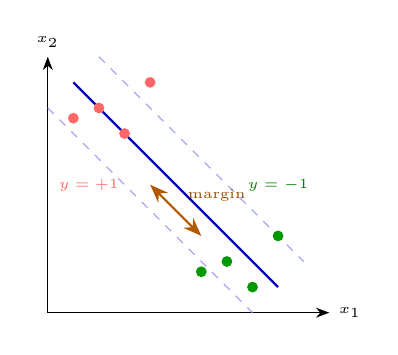
\begin{tikzpicture}[>=Stealth, scale=0.65]
  % Axes
  \draw[->] (0,0) -- (5.5,0) node[right] {\tiny $x_1$};
  \draw[->] (0,0) -- (0,5) node[above] {\tiny $x_2$};

  % Decision boundary
  \draw[thick, blue!70!black] (0.5, 4.5) -- (4.5, 0.5);

  % Margin lines
  \draw[dashed, blue!40] (0, 4.0) -- (4.0, 0);
  \draw[dashed, blue!40] (1.0, 5.0) -- (5.0, 1.0);

  % Class +1 (above)
  \fill[red!60] (1.0, 4.0) circle (3pt);
  \fill[red!60] (1.5, 3.5) circle (3pt);
  \fill[red!60] (2.0, 4.5) circle (3pt);
  \fill[red!60] (0.5, 3.8) circle (3pt);

  % Class -1 (below)
  \fill[green!60!black] (3.5, 1.0) circle (3pt);
  \fill[green!60!black] (4.0, 0.5) circle (3pt);
  \fill[green!60!black] (4.5, 1.5) circle (3pt);
  \fill[green!60!black] (3.0, 0.8) circle (3pt);

  % Labels
  \node[font=\tiny, red!60] at (0.8, 2.5) {$y=+1$};
  \node[font=\tiny, green!50!black] at (4.5, 2.5) {$y=-1$};

  % Margin annotation
  \draw[<->, thick, orange!70!black] (2.0, 2.5) -- (3.0, 1.5);
  \node[font=\tiny, orange!60!black] at (3.3, 2.3) {margin};
\end{tikzpicture}
\end{center}

\vspace{0.3em}
\begin{alertblock}{Design Goal}
Binary linear SVM with \textbf{Pegasos-style online SGD},
hinge loss, and L2 regularization. Labels are $\{+1, -1\}$.
\end{alertblock}
\end{column}
\end{columns}
\end{frame}

% ===========================================================================
\section{Algorithm Theory}
% ===========================================================================

\begin{frame}{Linear SVM with Hinge Loss}
\begin{columns}[T]
\begin{column}{0.48\textwidth}
\textbf{Decision function:}
\[
  f(\mathbf{x}) = w_0 + \sum_{i=1}^{n} w_i \cdot x_i
\]

\textbf{Prediction:}
\[
  \hat{y} = \begin{cases} +1 & \text{if } f(\mathbf{x}) \geq 0 \\ -1 & \text{otherwise} \end{cases}
\]

\textbf{Hinge loss + L2 regularization:}
\[
  L = \max(0, 1 - y \cdot f(\mathbf{x})) + \frac{\lambda}{2}\|\mathbf{w}\|^2
\]

\vspace{0.3em}
\textbf{SGD update} (Pegasos):
\begin{itemize}
  \item If $y \cdot f(\mathbf{x}) < 1$ (margin violation):\\
    $w_j \leftarrow w_j + \eta(y \cdot x_j - \lambda \cdot w_j)$
  \item Otherwise (correct side of margin):\\
    $w_j \leftarrow w_j - \eta \cdot \lambda \cdot w_j$
\end{itemize}
\end{column}

\begin{column}{0.48\textwidth}
\begin{center}
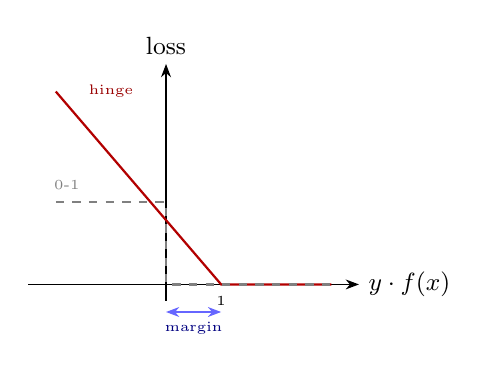
\begin{tikzpicture}[>=Stealth, scale=0.7]
  % Axes
  \draw[->] (-2.5,0) -- (3.5,0) node[right] {\small $y \cdot f(x)$};
  \draw[->] (0,-0.3) -- (0,4) node[above] {\small loss};

  % Hinge loss
  \draw[thick, red!70!black] (-2, 3.5) -- (1, 0) -- (3, 0);

  % 0-1 loss (step)
  \draw[thick, gray, dashed] (-2, 1.5) -- (0, 1.5) -- (0, 0) -- (3, 0);

  % Labels
  \node[font=\tiny] at (1, -0.3) {1};
  \node[font=\tiny, red!60!black] at (-1, 3.5) {hinge};
  \node[font=\tiny, gray] at (-1.8, 1.8) {0-1};

  % Margin annotation
  \draw[<->, thin, blue!60] (0, -0.5) -- (1, -0.5);
  \node[font=\tiny, blue!50!black] at (0.5, -0.8) {margin};
\end{tikzpicture}
\end{center}

\vspace{0.3em}
\begin{block}{Key Properties}
\begin{itemize}
  \item Hinge loss is convex and subdifferentiable
  \item L2 regularization prevents overfitting
  \item $\lambda$ controls margin width vs. accuracy
  \item Online update: one sample at a time
\end{itemize}
\end{block}
\end{column}
\end{columns}
\end{frame}

% ===========================================================================
\section{Data Structure}
% ===========================================================================

\begin{frame}[fragile]{The \texttt{tiku\_kits\_ml\_linsvm} Structure}
\begin{columns}[T]
\begin{column}{0.48\textwidth}
\begin{lstlisting}[style=cstyle,
  title={ml/classification/tiku\_kits\_ml\_linsvm.h}]
struct tiku_kits_ml_linsvm {
    /* bias + feature weights Q(shift) */
    int32_t weights[
        TIKU_KITS_ML_LINSVM_MAX_FEATURES
        + 1];
    uint8_t  n_features;
    uint8_t  shift;
    int32_t  learning_rate;
    int32_t  lambda;
    uint16_t n;
};
\end{lstlisting}

\textbf{Memory footprint:}\\
$(8+1) \times 4 + 1 + 1 + 4 + 4 + 2 = 48$ bytes.\\
All statically allocated --- no heap.
\end{column}

\begin{column}{0.48\textwidth}
\begin{lstlisting}[style=cstyle,
  title={Defaults at init (Q8)}]
/* Learning rate: ~0.1 */
lr = (1 << shift) / 10;   /* = 25 */

/* Regularization: ~0.01 */
lambda = (1 << shift) / 100; /* = 2 */
\end{lstlisting}

\vspace{0.5em}
\begin{block}{Labels: $\{+1, -1\}$}
Unlike logistic regression ($\{0, 1\}$), SVM uses
$y \in \{+1, -1\}$. The \texttt{train()} function
validates this --- rejects any other label value.
\end{block}

\vspace{0.3em}
\begin{block}{Decision Margin}
\texttt{decision()} returns the \textbf{raw signed margin}
$f(\mathbf{x})$. Large positive = confident $+1$;
large negative = confident $-1$.
\end{block}
\end{column}
\end{columns}
\end{frame}

% ===========================================================================
\section{API Reference}
% ===========================================================================

\begin{frame}[fragile]{Complete API}
\begin{table}
\centering
\small
\begin{tabular}{@{}lp{8cm}@{}}
\toprule
\textbf{Function} & \textbf{Description} \\
\midrule
\texttt{tiku\_kits\_ml\_linsvm\_init(svm, nf, sh)}
  & Initialize with \texttt{nf} features, Q-format \texttt{sh} \\
\texttt{tiku\_kits\_ml\_linsvm\_reset(svm)}
  & Zero all weights, reset training count \\
\texttt{tiku\_kits\_ml\_linsvm\_set\_lr(svm, rate)}
  & Set learning rate in Q(shift) \\
\texttt{tiku\_kits\_ml\_linsvm\_set\_lambda(svm, lam)}
  & Set L2 regularization strength \\
\midrule
\texttt{tiku\_kits\_ml\_linsvm\_train(svm, x, y)}
  & One Pegasos SGD step; label $y \in \{+1,-1\}$ \\
\texttt{tiku\_kits\_ml\_linsvm\_predict(svm, x, \&result)}
  & Binary prediction: $+1$ or $-1$ \\
\texttt{tiku\_kits\_ml\_linsvm\_decision(svm, x, \&margin)}
  & Raw signed margin $f(\mathbf{x})$ in Q(shift) \\
\midrule
\texttt{tiku\_kits\_ml\_linsvm\_get\_weights(svm, w)}
  & Export weight vector (bias + features) \\
\texttt{tiku\_kits\_ml\_linsvm\_set\_weights(svm, w)}
  & Load pre-trained weights \\
\texttt{tiku\_kits\_ml\_linsvm\_count(svm)}
  & Number of training samples seen \\
\bottomrule
\end{tabular}
\end{table}

\vspace{0.3em}
\begin{alertblock}{Labels Must Be $\pm 1$}
\texttt{train()} returns \texttt{ERR\_PARAM} if $y$ is not exactly
$+1$ or $-1$. This differs from logistic regression which uses $\{0, 1\}$.
\end{alertblock}
\end{frame}

% ===========================================================================
\section{Implementation Details}
% ===========================================================================

\begin{frame}[fragile]{Pegasos SGD Training}
\begin{lstlisting}[style=cstyle,
  title={tiku\_kits\_ml\_linsvm.c --- train (simplified)}]
int tiku_kits_ml_linsvm_train(struct tiku_kits_ml_linsvm *svm,
                              const tiku_kits_ml_elem_t *x, int8_t y)
{
    int32_t margin;
    int64_t lr_q = (int64_t)svm->learning_rate;
    int32_t one_q = (int32_t)(1 << svm->shift);

    margin = dot_product(svm, x);   /* f(x) in Q(shift) */

    if ((int64_t)y * (int64_t)margin < (int64_t)one_q) {
        /* Margin violation: hinge loss gradient */
        for (i = 0; i < svm->n_features; i++) {
            svm->weights[i + 1] +=
                (int32_t)((lr_q * ((int64_t)y * (int64_t)x[i]
                          - ((int64_t)svm->lambda * (int64_t)svm->weights[i + 1])
                            >> svm->shift)) >> svm->shift);
        }
    } else {
        /* Correct side: regularization only */
        for (i = 0; i < svm->n_features; i++) {
            svm->weights[i + 1] -=
                (int32_t)((lr_q * (int64_t)svm->lambda
                          * (int64_t)svm->weights[i + 1])
                          >> (2 * svm->shift));
        }
    }
    return TIKU_KITS_ML_OK;
}
\end{lstlisting}
\end{frame}

% ===========================================================================
\section{Examples}
% ===========================================================================

\begin{frame}[fragile]{Example 1: Temperature Threshold}
\begin{lstlisting}[style=cstyle,
  title={examples/example\_ml\_linsvm.c --- hot/cold binary classification}]
struct tiku_kits_ml_linsvm svm;
int8_t result;

tiku_kits_ml_linsvm_init(&svm, 1, 8);   /* 1 feature, Q8 */

/* Train: cold(-1) / hot(+1) */
static const int32_t temps[]  = {150, 180, 200, 300, 320, 350};
static const int8_t labels[]  = { -1,  -1,  -1,  +1,  +1,  +1};

uint8_t epoch, s;
for (epoch = 0; epoch < 20; epoch++) {
    for (s = 0; s < 6; s++) {
        tiku_kits_ml_linsvm_train(&svm, &temps[s], labels[s]);
    }
}

/* Predict */
int32_t reading = 280;
tiku_kits_ml_linsvm_predict(&svm, &reading, &result);
/* result: +1 (hot) or -1 (cold) */
\end{lstlisting}
\end{frame}

% ---------------------------------------------------------------------------
\begin{frame}[fragile]{Example 2: Motion Detection with Margin}
\begin{columns}[T]
\begin{column}{0.52\textwidth}
\begin{lstlisting}[style=cstyle,
  title={2-D with decision margin}]
struct tiku_kits_ml_linsvm svm;
int8_t result;
int32_t margin;

tiku_kits_ml_linsvm_init(&svm, 2, 8);

/* Train on accelerometer data */
/* ... training loop ... */

/* Classify and inspect margin */
tiku_kits_ml_elem_t sample[] = {15, 20};
tiku_kits_ml_linsvm_predict(&svm,
    sample, &result);
tiku_kits_ml_linsvm_decision(&svm,
    sample, &margin);

/* margin: signed distance in Q8 */
if (margin > 128) {
    /* Confident positive (> 0.5) */
    trigger_motion_alert();
} else if (margin < -128) {
    /* Confident negative */
    enter_sleep_mode();
} else {
    /* Uncertain: sample more */
    request_more_data();
}
\end{lstlisting}
\end{column}

\begin{column}{0.44\textwidth}
\begin{center}
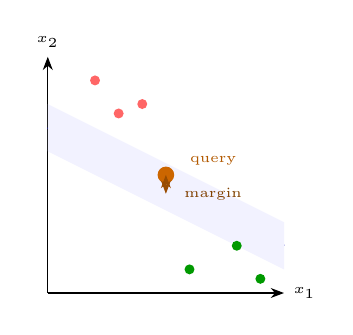
\begin{tikzpicture}[>=Stealth, scale=0.6]
  \draw[->] (0,0) -- (5,0) node[right] {\tiny $x_1$};
  \draw[->] (0,0) -- (0,5) node[above] {\tiny $x_2$};

  % Decision boundary
  \draw[thick, blue!70!black] (0, 3.5) -- (5, 1);

  % Margin zones
  \fill[blue!5] (0, 3.0) -- (5, 0.5) -- (5, 1.5) -- (0, 4.0) -- cycle;

  % Points
  \fill[red!60] (1, 4.5) circle (3pt);
  \fill[red!60] (2, 4.0) circle (3pt);
  \fill[red!60] (1.5, 3.8) circle (3pt);
  \fill[green!60!black] (3, 0.5) circle (3pt);
  \fill[green!60!black] (4, 1.0) circle (3pt);
  \fill[green!60!black] (4.5, 0.3) circle (3pt);

  % Query
  \fill[orange!80!black] (2.5, 2.5) circle (5pt);
  \node[font=\tiny, orange!70!black] at (3.5, 2.8) {query};
  \draw[<->, thin, orange!60!black] (2.5, 2.5) -- (2.5, 2.1);
  \node[font=\tiny, orange!50!black] at (3.5, 2.1) {margin};
\end{tikzpicture}
\end{center}

\vspace{0.5em}
\begin{block}{Margin as Confidence}
The absolute margin $|f(\mathbf{x})|$ indicates
distance from the decision boundary.
Large margin = high confidence.
Use it for confidence-aware decisions.
\end{block}
\end{column}
\end{columns}
\end{frame}

% ===========================================================================
\section{Test Suite}
% ===========================================================================

\begin{frame}{Test Cases Overview}
\begin{table}
\centering
\small
\begin{tabular}{@{}clp{7cm}@{}}
\toprule
\textbf{\#} & \textbf{Test Function} & \textbf{What It Verifies} \\
\midrule
1 & \texttt{test\_kits\_ml\_linsvm\_init}
  & Proper initialization, parameter validation \\
2 & \texttt{test\_kits\_ml\_linsvm\_pretrained}
  & Pre-loaded weights produce correct $\pm 1$ \\
3 & \texttt{test\_kits\_ml\_linsvm\_decision}
  & Raw decision margin sign and magnitude \\
4 & \texttt{test\_kits\_ml\_linsvm\_training}
  & SGD convergence on linearly separable data \\
5 & \texttt{test\_kits\_ml\_linsvm\_two\_features}
  & 2-D classification \\
6 & \texttt{test\_kits\_ml\_linsvm\_learning\_rate}
  & Custom learning rate accepted \\
7 & \texttt{test\_kits\_ml\_linsvm\_lambda}
  & Custom regularization strength \\
8 & \texttt{test\_kits\_ml\_linsvm\_reset}
  & Reset clears weights and count \\
9 & \texttt{test\_kits\_ml\_linsvm\_null\_inputs}
  & All functions reject NULL with ERR\_NULL \\
\bottomrule
\end{tabular}
\end{table}
\end{frame}

% ===========================================================================
\section{Summary}
% ===========================================================================

\begin{frame}{Summary}
\begin{columns}[T]
\begin{column}{0.48\textwidth}
\begin{block}{What We Built}
\begin{itemize}
  \item Binary linear SVM classifier
  \item Pegasos-style online SGD
  \item Hinge loss + L2 regularization
  \item 48 bytes of state, no heap
  \item Raw margin output for confidence
\end{itemize}
\end{block}

\begin{block}{Key Design Choices}
\begin{itemize}
  \item \texttt{int64\_t} dot product prevents overflow
  \item Labels $\{+1, -1\}$ (validated)
  \item Separate \texttt{predict()} and \texttt{decision()}
  \item Tunable $\lambda$ for regularization strength
\end{itemize}
\end{block}
\end{column}

\begin{column}{0.48\textwidth}
\begin{block}{Use Cases}
\begin{itemize}
  \item Temperature threshold classification
  \item Motion/vibration binary detection
  \item Margin-based confidence decisions
  \item Noise-robust sensor classification
\end{itemize}
\end{block}

\begin{block}{Files}
\scriptsize
\begin{tabular}{@{}lp{4.5cm}@{}}
Header: & \texttt{ml/classification/tiku\_kits\_ml\_linsvm.h} \\
Source: & \texttt{ml/classification/tiku\_kits\_ml\_linsvm.c} \\
Tests: & \texttt{tests/ml/test\_kits\_ml\_linsvm.c} \\
Example: & \texttt{examples/example\_ml\_linsvm.c} \\
\end{tabular}
\end{block}
\end{column}
\end{columns}
\end{frame}

% ---------------------------------------------------------------------------
\begin{frame}{Thank You}
\begin{center}
\Large\textbf{TikuKits ML: Linear SVM}\\[0.5em]
\normalsize Integer-Only Machine Learning for Physical AI Endpoints\\[1.5em]

\begin{tabular}{rl}
  Repository: & \url{https://github.com/tikuos/tikuOS} \\
  License:    & Apache 2.0 \\
  Common:     & \texttt{tikukits/ml/tiku\_kits\_ml.h} \\
  Header:     & \texttt{tikukits/ml/classification/tiku\_kits\_ml\_linsvm.h} \\
  Source:     & \texttt{tikukits/ml/classification/tiku\_kits\_ml\_linsvm.c} \\
  Tests:      & \texttt{tikukits/tests/ml/test\_kits\_ml\_linsvm.c} \\
  Examples:   & \texttt{tikukits/examples/example\_ml\_linsvm.c} \\
\end{tabular}
\end{center}
\end{frame}

\end{document}
